\documentclass[11pt, letterpaper, twoside]{article}
\usepackage[letterpaper, portrait, left=1in, right=1in, top=1in, bottom=1in]{geometry}\usepackage{amsmath}
\usepackage{amssymb}
\usepackage{graphicx}
\usepackage[explicit]{titlesec} %Alternate titlepage, gives \begin{titlepage} command
\usepackage{epstopdf} %No clue what this is
\usepackage{amsmath} %This is also needed
\usepackage{inputenc} %don't remember what this is for
\usepackage{enumitem} % For alphabetical labels
\usepackage{booktabs, multirow} %for borders and merged ranges
\usepackage{soul}% for underlines
\usepackage[table]{xcolor} % for cell colors
\newcommand\aug{\fboxsep=-\fboxrule\!\!\!\fbox{\strut}\!\!\!} %Use \aug to make a equal column (|) for an augmented matrix
\begin{document}
\begin{titlepage}
	\centering
	\vspace*{60px}
	\hspace{0pt}
	
\includegraphics[width=0.2\textwidth]{logo}\par\vspace{1cm}
	{\scshape\LARGE Athabasca University \par}
	\vspace{1cm}
	{\scshape\Large MATH 265\par}
	\vspace{1.5cm}
	{\huge\bfseries Assignment 2\par}
	\vspace{2cm}
	{\Large\itshape Stanley Zheng\par}
	\vfill
	{\large July 2, 2020\par}
	\vspace*{50px}
	\hspace{0pt}
\pagebreak
\end{titlepage}
\begin{enumerate}
\item \begin{enumerate}[label=(\alph*)] %Q1
\item %Q1A
$x=30\tan(\theta)$
\item %Q1B
$\theta \in \mathbb{R}, [0, \frac{\pi}{2})$
\item %Q1C
We have $\theta=\frac{\pi}{3}$. Plugging in, we get $x=30\tan(\frac{\pi}{3})=\boxed{30\sqrt3m}$
\end{enumerate}
\item \begin{enumerate}[label=(\alph*)]%Q2
\item %Q2A
\begin{tabular}[t]{ |c|c|c|c|c|c|c|c|c| }
\hline
$x$ & -2 & -1 & 0 & 1 & 2 & 3 & 4 & 5 \\
\hline
$f(x)$ & 0 & -0.25 & -0.5 & -2 & -1 & 0 & 1 & 2\\
\hline
$g(x)$ & 2 & 2 & 2 & 1 & 0 & -1 & -2 &\\
\hline
\end{tabular}
\item \begin{enumerate}[label=\roman*.]
\item $g\circ f(-2) = g(f(-2))=g(0)=2$
\item $g\circ f(1)= g(f(1))=g(-2)=2$
\item $g\circ f(4) = g(f(4))=g(1)=1$
\item $f\circ g(0) = f(g(0))=f(2)=-1$
\item $f\circ g(4) = f(g(4))=f(-2)=0$
\item $f\circ g(-1) = f(g(-1))=f(2)=-1$
\end{enumerate}
\end{enumerate}
\item \begin{enumerate}[label=(\alph*)] %Q3
\item Since $\frac{f}{g}=fg^{-1}$, we have%Q3A
\begin{align*}
fg^{-1}&=(\sqrt{1-2x})\left( \frac{x}{x^2-1}\right)^{-1}\\
&= \frac{\sqrt{1-2x}(x^2-1)}{x}
\end{align*}
Therefore our domain is $(-\infty, 0)\cup (0, \frac{1}{2}], x \in \mathbb{R}$
\item %Q3B
\begin{align*}
g\circ f &= g(f(x))\\
&=\frac{\sqrt{1-2x}}{(\sqrt{1-2x})^2-1}\\
&=\frac{\sqrt{1-2x}}{-2x}
\end{align*}
The domain of this function is still $(-\infty, 0)\cup(0, \frac{1}{2}], x\in\mathbb{R}$
\item %Q3C
\begin{align*}
gf^2&=g(x)\cdot f(x)^2\\
&=\left(\frac{x}{x^2-1}\right)(\sqrt{1-2x})^2\\
&=\frac{x-2x^2}{x^2-1}\\
&=\frac{x-2x^2}{(x-1)(x+1)}
\end{align*}
The domain for $gf^2$ is $(-\infty, -1)\cup(-1, \frac{1}{2}]$
\end{enumerate}
\item \begin{enumerate}[label=(\alph*)]%Q4
\item %Q4A
We begin our manipulations by horizontally stretching our graph by a factor of $\frac{1}{2}$. Next, we translate our graph down one unit. Our final transformed graph is as follows:
\newline 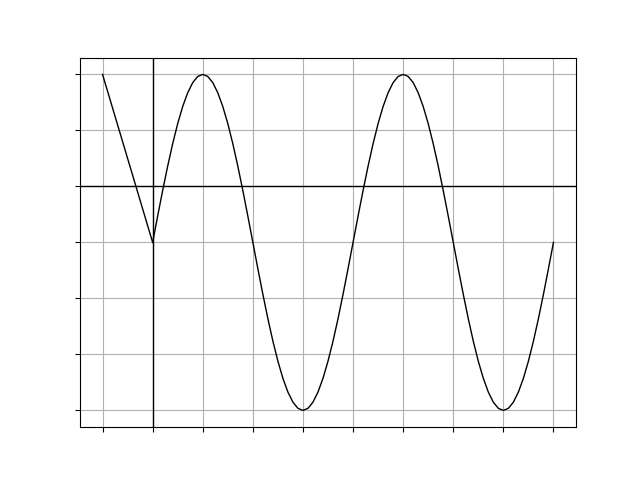
\includegraphics[width=0.5\textwidth]{q4a}
\item %Q4B
We first reflect our graph accross the $x$ axis, then vertically stretch it by a factor of $2$. Next, we translate one unit up. Our final transformed graph is as follows:
\newline 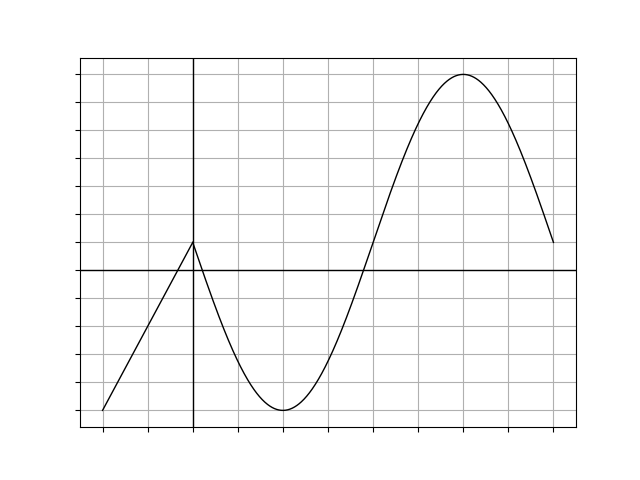
\includegraphics[width=0.5\textwidth]{q4b}
\end{enumerate}
\item \begin{enumerate}[label=(\alph*)]%Q5
\item %Q5A
The limit is well defined. As $x$ approaches 2 frome either the right or left side, $y$ approaches 0.
\item %Q5B
The limit is not defined. First calculating $\lim_{x\to \infty}\frac{x^2+1}{x+3}$, we can divide each side by the highest denominator power, $x$. $\frac{x+\frac{1}{x}}{1+\frac{3}{x}}$. The numerator is $\infty$, and the denominator is $1$. Since $\cot (\infty)$ is not defined, our limit is not defined.
\end{enumerate}
\item \begin{enumerate}[label=(\alph*)] %Q6
\item %Q6A
Step 2 is incorrect. We have $\lim_{x\to -\infty}\frac{\sqrt{x^2-x^3}}{x}$, and we can factor the numerator into $\lim_{x\to -\infty}\frac{\sqrt{x^2}\sqrt{1-x}}{x}$. Then, simplifying, we have $\lim_{x\to -\infty}-\sqrt{1-x}$.\\

We know that $\lim_{x\to -\infty} \sqrt{1-x}$ is infinite, and therefore, $\lim_{x\to - \infty} \sqrt {1-x}$ is infinite, therefore, $\lim_{x\to -\infty}\frac{\sqrt{x^2-x^3}}{x}=\boxed{-\infty}$

\item %Q6B
The fourth step is incorrect. The first two limits are correct, however, a mistake was made for $\lim_{x\to0} 1+\cos(3x)$. Since $\cos(3x)=1$, we know that $\lim_{x\to0} 1+\cos(3x)=2$. Therefore, the correct answer is $\boxed{-\frac{2}{9}}$ 
\end{enumerate}
\item\begin{enumerate}[label=(\alph*)] %Q7
\item %Q7A
We can simply plug in $x=0$. $\lim_{x\to0}\frac{\sin(\pi-x)}{\sqrt{x^2-x+1}}=\frac{sin(\pi-0)}{\sqrt{0^2-0+1}}=\sin\pi=\boxed{0}$
\item %Q7B
We can begin by simplifying the fraction.
$$\lim_{x\to3}\frac{x^3-3x^2+4x-12}{3x^2-7x-6}=\lim_{x\to3}\frac{(x-3)(x^2+4)}{(x-3)(3x+2)}$$
Finally, we can plug in $x=3$ and solve.
$$\lim_{x\to3}=\frac{x^2+4}{3x+2}=\frac{3^2+4}{3\cdot3+2}=\boxed{\frac{13}{11}}$$
\item %Q7C
We can start by expanding, then dividing the fraction by the highest denominator power, which is $x^3$.
\begin{align*}
\lim_{x\to\infty}\cos\left(\frac{(\pi x+1)(3-x^2)}{x^3-\pi}\right)&=\lim_{x\to\infty}\cos\left(\frac{-\pi x^3-x^2+3\pi x+3}{x^3-\pi}\right)\\
&=\lim_{x\to\infty}\cos\left( \frac{-\pi-\frac{1}{x}+\frac{3\pi}{x^2}+\frac{3}{x^3}}{1-\frac{\pi}{x^3}}\right)\\
&= \cos -\pi \\
&= \boxed{-1}
\end{align*}
\item %Q7D
Again, we can find the limit by dividing by the highest denominator power, $x^2.$
$$\lim_{x\to \infty}\frac{x\sin(3x)}{x^2+1}=\frac{\frac{\sin(3x)}{x}}{1+\frac{1}{x^2}}$$
We can now evaluate the limit of the numerator and denominator separately. The denominator is $\lim_{x\to\infty}1+\frac{1}{x^2}=1+0=1$. Since $\sin 3x$ is between 1 and -1, and by sandwich theorem, $-\frac{1}{x}\leq \frac{\sin 3x}{x}\leq \frac{1}{x}$, the numerator is 0. Therefore, we have $\lim_{x\to \infty}\frac{x\sin(3x)}{x^2+1}=\boxed{0}$.
\item %Q7E
We can begin by rationalizing the numerator.
$$\lim_{x\to1^+}\sin\left(\frac{\sqrt{x+1}}{x^2-1}\right)=\lim_{x\to1^+}\sin\left(\frac{1}{(x-1)\sqrt{x+1}}\right)$$
The denominator and numerator are positive and the denominator approaches 0 as $x$ approaches 1 from the right. As such, the fraction approaches $\infty$. 
Then, $\lim_{x\to1^+} \sin\left(\frac{\sqrt{x+1}}{x^2-1}\right)$ is convergent and undefined since sine is a convergent function and $\lim_{\theta\to\infty}\sin\theta$ is undefined.
\item %Q7F
We can start by dividing the fraction by the highest denominator power, $\sqrt{x+1}$.
$$\lim_{x\to0^+} \frac{\sqrt{x^3+x^2}}{\sqrt{x+1}-1}=\frac{x}{1-{\frac{1}{\sqrt{x+1}}}}$$
Next, we can rationalize
$$\lim_{x\to0^+}\left(\frac{x}{1-{\frac{1}{\sqrt{x+1}}}}\right)\left(\frac{1+\frac{1}{\sqrt{x+1}}}{1+\frac{1}{\sqrt{x+1}}}\right)=\lim_{x\to0^+} x+\sqrt{x+1}+1$$
Finally, we can plug in 0 to $x+\sqrt{x+1}+1$. $0+\sqrt{1+0}+1=\boxed{2}$
\item %Q7G
We know that $\cos(2x)=\cos^2(x)-\sin^2(x)$ and that $\cos^2(x)=1-\sin^2(x)$. Substituting this into the equation, we have
\begin{align*}
\lim_{x\to0}\frac{\sin^2(3x)}{1-\cos(2x)}&=\lim_{x\to0}\frac{\sin^2(3x)}{1-(1-2\sin^2(2x))}\\
&=\lim_{x\to0}\frac{\sin^2(3x)}{2\sin^2x}\\
&=\frac{1}{2}\lim_{x\to0}\left(\frac{\sin(3x)}{\sin x}\right)^2
\end{align*}
We know that $\lim_{x\to 0}\frac{\sin (x)}{x}=1$, so we will try to manipulate our limit into it. To do this, we divide the numerator and denominator of the fraction by $x$.
$$\frac{1}{2}\lim_{x\to0}\left(\frac{\frac{\sin(3x)}{x}}{\frac{\sin (x)}{x}}\right)^2$$
Next, we multiply the numerator by 3 and divide it by 3.
$$\frac{1}{2}\lim_{x\to0}\left(\frac{3\frac{\sin(3x)}{3x}}{\frac{\sin (x)}{x}}\right)^2$$
We can then move the 3 out of the brackets and find the limit of the numerator and denominator individually.
$$\frac{9}{2}\left(\frac{\lim_{x\to0}\frac{\sin(3x)}{3x}}{\lim_{x\to0}\frac{\sin(x)}{x}}\right)^2$$
$$\frac{9}{2}\left(\frac{1}{1}\right)^2=\boxed{4.5}$$
\end{enumerate}
\item\begin{enumerate}[label=(\alph*)] %Q8
\item %Q8A
$\lim_{x\to0^-}f(x)$ approaches from the left side of 0, so therefore, $f(x)=\frac{2}{x}$. Then, we have $\lim_{x\to0^-}\frac{2}{x}$, which is $\boxed{\infty}$.
\item %Q8B
$\lim_{x\to0^+}f(x)$ approaches from the right side of 0, so therefore, we have

$\lim_{x\to0}\sqrt x+\cos(\pi x)$. Plugging in $x=0$, we have $\sqrt0+\cos(\pi\cdot0)=\cos(0)=\boxed{1}$
\item %Q8C
$\lim_{x\to5^-}f(x)$ approaches from the left side of 5, so we have

$\lim_{x\to5}\sqrt x+\cos(\pi x)$. Simply plugging in $x=5$, we have $\sqrt5+\cos(\pi\cdot5)=\boxed{\sqrt5-1}$
\item %Q8D
$\lim_{x\to5^+}f(x)$ approaches from the right side of 5, so we have

$\lim_{x\to5+}\frac{x}{x-5}$. To solve this limit, we first divide by the numerator's largest power, $x$.
$$\lim_{x\to5+}\frac{1}{x-\frac{5}{x}}$$
The denominator approaches 0 as $x$ approaches 5, so we know that this limit approaches infinity.
\item %Q8E
This limit does not exist. Depending on which side the limit is approached from, the limit approaches different values. Specifically, we found $\lim_{x\to5^+}f(x)=\sqrt5-1$, but $\lim_{x\to5^-}f(x)=\infty$.
\item %Q8F
According to the piecewise function, our limit is equivalent to $\lim_{x\to\infty}\frac{x}{x-5}$. To solve this limit, we can divide by the largest denominator fraction, $x$.
$$\lim_{x\to\infty} \frac{1}{1-\frac{5}{x}}$$
We can now see that the denominator approaches 1 as $x$ approaches infintiy. As a result, our limit is equal to 1.
\item %Q8G
From the piecewise function, our limit is equivalent to $\lim_{x\to -\infty} \frac{2}{x}$. Since we have infinity as a denominator, our limit aproaches 0.
\end{enumerate}
This function is not continuous at $x=0, 5$. This can be seen in the limits we calculated in this question, where $\lim_{x\to0^-}$ and $\lim_{x\to0^+}$ as well as $\lim_{x\to5^-}$ and $\lim_{x\to5^+}$ had different values.
\item%Q9
In order to make a single function that fulfills these conditions, we need to create a piecewise function. We can arrive at a few conclusions from the provided conditions. Firstly, our graph needs to pass through points (5, 6) and (-5, 6). Next, we need a positive asymptote on the left side of 0, and a graph with a negative slope after point (5,6) on the right side.
$$
f(x) =
\begin{cases}

-\frac{1}{x}+5 & -5< x < 0 \\
\frac{6}{5}x & 0< x < 5\\
-x & 5 \leq x
\end{cases}
$$
The graph of this function which satisfies all of these conditions needs to have a zero, where $f(x)=0$, since condition $f$ specifies that $\lim_{x\to0}f(x)=0$, condition $c$ specifies $f(-5)=f(5)$, and condition $d$ specifies $\lim_{x\to5}f(x)=6$. Finally, condition $g$ specifies that $\lim_{x\to\infty}f(x)=-\infty$. This means that the function must near the origin, have a positive slope going up to point (5,6), then have a negative slope after this point going down to negative infinity. As such, there must be a zero somewhere between (5,6) and negative infinity to fulfill all of the conditions.
\newline 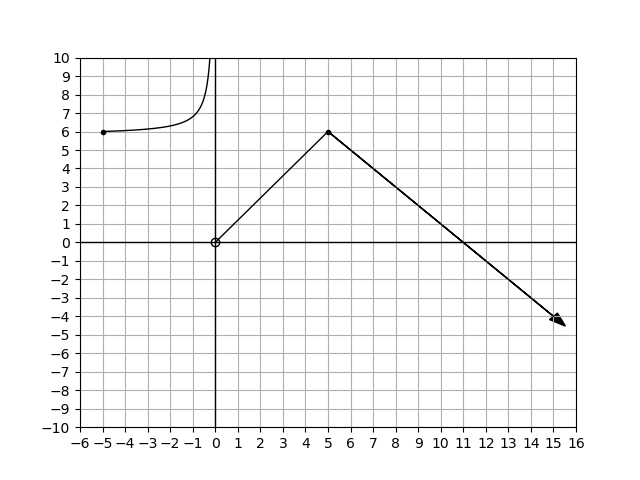
\includegraphics[width=0.5\textwidth]{q9}
\item \begin{enumerate}[label=(\alph*)] %Q10
\pagebreak \item %Q10A
For $\varepsilon>0, \delta>0, 0<|x-a|<\delta$, 

$$|f(x)-L|<\varepsilon$$

$$c|f(x)-L|<c\varepsilon$$

$$|cf(x)-cL|<\varepsilon^\prime, \varepsilon^\prime=c\varepsilon>0$$

$$\lim_{x\to a}f(x)=cL, (=L^\prime, c^\prime=cL)$$

Now, $\lim_{x\to\infty} f(x)=-\infty$

$\therefore \lim_{x\to\infty}f(x)=c(-\infty)=-\infty$\\

\item %Q10b
% Since we are working with infinite limits, we can use the formal definition of a limit as follows: \\
% $\lim_{x\to\infty}g(x)=\infty$ if for every number $\varepsilon>0$, there is a number $\delta>0$ such that $g(x)>\varepsilon$ whenever $x>\delta$.

% We are given $g(x)\le f(x)$. Therefore, we have $f(x)\geq g(x)>\varepsilon$ whenever $x>\delta>0$. As a result, if $\lim_{x\to a}g(x)=\infty$, then $\lim_{x\to a}=\infty$.
% \\

% Alternate proof:
For $\varepsilon>0$, whenever $\delta>0$, $0<|x-a|<\delta$, and $|g(x)-L|<\varepsilon$
$$-\varepsilon<g(x)-L<\varepsilon$$
$$g(x)-L<\varepsilon$$
As $x\to A$, $f(x)\geq g(x)$
$$\therefore f(x)-L<\varepsilon^\prime , \varepsilon^\prime>\varepsilon>0$$
We also have $f(x)\geq g(x)$. Since $g(x)-L>-\varepsilon$, 
$$f(x)-L\geq g(x)-L>-\varepsilon$$
Since $\varepsilon^\prime$, we have $\varepsilon>-\varepsilon^\prime$
$$\therefore f(x)-L>-\varepsilon^\prime$$

\end{enumerate}
\end{enumerate}
\end{document}
